\subsection{Embedding Words in Non-Vector Space with Unsupervised Graph Learning}
\begin{center}
  \begin{tabular}{rl}
  % after \\: \hline or \cline{col1-col2} \cline{col3-col4} ...
  论文地址:& \href{https://arxiv.org/abs/2010.02598}{https://arxiv.org/abs/2010.02598} \\
  源码地址:& \href{https://github.com/yandex-research/graph-glove}{graph-glove} \\
  关键词:& \textbf{embedding, representation learning} \\
  写于:& \date{2020-10-08}
  \end{tabular}
\end{center}
传统的word embedding通常是将词嵌入到向量空间中,\cite{10.1145/219717.219748}指出words可以形成具有隐式层次结构的图,词向量的质量与选取什么样的向量空间有很大的关系。针对这个问题,该论文\cite{ryabinin2020embedding}提出了GraphGlove,将词嵌入到带权图(weighted graph)中。在word相似性及相关任务中,该论文提出的方法取得了比嵌入到向量空间中更好的效果。\\
\textbf{方法---GraphGlove}\hspace{6pt} 每个word视作带权图(weighted graph)中的一个结点,\textbf{词之间的距离使用图中结点之间的shortest path来表示(与欧氏空间中距离的定义不同)}。使用PRODIGE\cite{mazur2019vector}从数据中学习,可以得到一个带权图以及图中边的权重;再将学习得到的带权图用于GloVe\cite{pennington-etal-2014-glove}算法,学习得到在非欧空间中的词向量,关键之处是替换GloVe的损失函数中词之间距离为图中结点之间的最短距离。\\
该论文与其他embedding方法不同的之处:将word嵌入到非欧空间,学习到的带权图就是这个非欧空间。


\subsection{Accurate, Efficient and Scalable Training of Graph Neural Networks}
\begin{center}
  \begin{tabular}{rp{6cm}lp{12cm}}%{rl}
  % after \\: \hline or \cline{col1-col2} \cline{col3-col4} ...
  论文地址:& \href{https://arxiv.org/abs/2010.03166}{https://arxiv.org/abs/2010.03166} \\
  源码地址:& \href{https://github.com/GraphSAINT/GraphSAINT}{GraphSAINT} \\
  关键词:& \textbf{GRL, GNN, Graph sampling,
  Graph partitioning, Memory optimization} \\
  写于:& \date{2020-10-08}
  \end{tabular}
\end{center}
该论文\cite{Zeng_2021}针对GNN的训练方法提出了一些改进算法,主要的改进点是:通过采样子图及关键步骤(如汇聚结点的特征)并行化。论文中针对多种GNN模型设计了多种并行策略。

\subsection{Learning to Represent Image and Text with Denotation Graph}
\begin{center}
  \begin{tabular}{rp{6cm}lp{10cm}}%{rl}
  % after \\: \hline or \cline{col1-col2} \cline{col3-col4} ...
  论文地址:& \href{https://arxiv.org/abs/2010.02949}{https://arxiv.org/abs/2010.02949} \\
  源码地址:& \href{https://shalab.usc.edu/DG/}{DG} \\
  关键词:& \textbf{embedding, multimodal,  Denotation Graph} \\
  写于:& \date{2020-10-08}
  \end{tabular}
\end{center}
该论文\cite{zhang2020learning}提出了一种表征多模态(图像+文本)数据的方法。存在着大量对齐的“视觉+文本”的数据,如包含描述的图片、视频、带字幕的电影等。学习如何表示这种视觉和文本存在明显的语义联系的数据是有很大引用价值的,如通过文本搜索图片、视频,为视频/图片添加描述,通过语言查询视频/图片中的信息,可视化的问答系统等。\\
\begin{figure}[h]
    \centering
    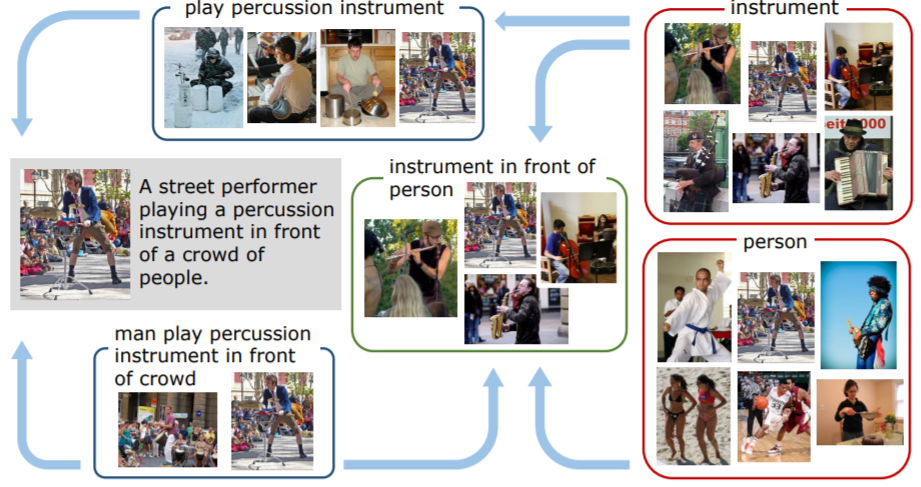
\includegraphics[width=.8\textwidth]{pics/DG.png}
    \caption{denotation graph extracted from the FLICKR30K dataset}
    \label{fig:DG}
\end{figure}
\textbf{方法}\hspace{6pt}论文中使用denotation graph(DG)\cite{young-etal-2014-image}来表示“图像+文本”的数据。该论文中的DG中每个结点包含一个文本描述和一系列与之对应的图像,图中的边是有向边,从语义上抽象的结点指向更具体地结点。如Fig.\ref{fig:DG}所示,DG中抽象的结点具有更一般的概念(如图中的person, instrument),抽象结点会指向更具体地结点(如play percussion instrument),每个结点会包含结点概念所对应的一些列图片。为什么要将文本与图像对应起来呢?论文中基于这样的一个假设:图片与文本对应的一致性有利于下游任务。在得到上述的DG(构建DG可参考\href{https://github.com/aylai/DenotationGraph}{这里}和\cite{young-etal-2014-image})后,在DG基础上学习图片和文本地表征。


\subsection{Towards Expressive Graph Representation}
\begin{center}
	\begin{tabular}{rp{6cm}lp{10cm}}%{rl}
		% after \\: \hline or \cline{col1-col2} \cline{col3-col4} ...
		论文地址:& \href{https://arxiv.org/abs/2010.05427}{https://arxiv.org/abs/2010.05427} \\
		源码地址:& \href{https://github.com/mocherson/Exp_GNN}{ExpGNN} \\
		关键词:& \textbf{GNN} \\
		写于:& \date{2020-10-13}
	\end{tabular}
\end{center}
该论文\cite{mao2020expressive}针对GNN存在的non-injective问题进行了改进,在理论上进行分析并设计了连续的、injectiv的邻居信息聚集函数,尽可能将不同的结点映射到不同的表征,相似的结点表征映射到相近的表征。聚集函数的{\color{red}连续性保证输入的微小变化能够导致表征的变化}。论文中对GNN中的邻居结点信息聚集函数、结点自身信息与聚集后的邻居信息结合函数、根据结点表征生成图表征的函数进行了设计,使其sh是injective且连续的。特别的针对邻居信息聚集函数,设计了两个版本,一个是固定的聚集函数,一个是被参数化的MLP。


\subsection{Enhancing Extractive Text Summarization with Topic-Aware Graph Neural Networks}
\begin{center}
	\begin{tabular}{rp{6cm}lp{10cm}}%{rl}
		% after \\: \hline or \cline{col1-col2} \cline{col3-col4} ...
		论文地址:& \href{https://arxiv.org/abs/2010.06253}{https://arxiv.org/abs/2010.06253} \\
		%源码地址:& \href{https://github.com/mocherson/Exp_GNN}{ExpGNN} \\
		关键词:& \textbf{Document Summarization, GAT, BERT} \\
		写于:& \date{2020-10-15}
	\end{tabular}
\end{center}
该论文\cite{cui2020enhancing}针对抽取式文本摘要问题提出了一个基于GNN的方法。现有的抽取式的文档摘要算法中,是通过从文档中抽取一个句子序列作为文档的摘要,但是通常没有考虑句子之间的关系,论文针对这个问题,提出了Topic-GraphSum模型。
\begin{figure}[h]
	\centering
	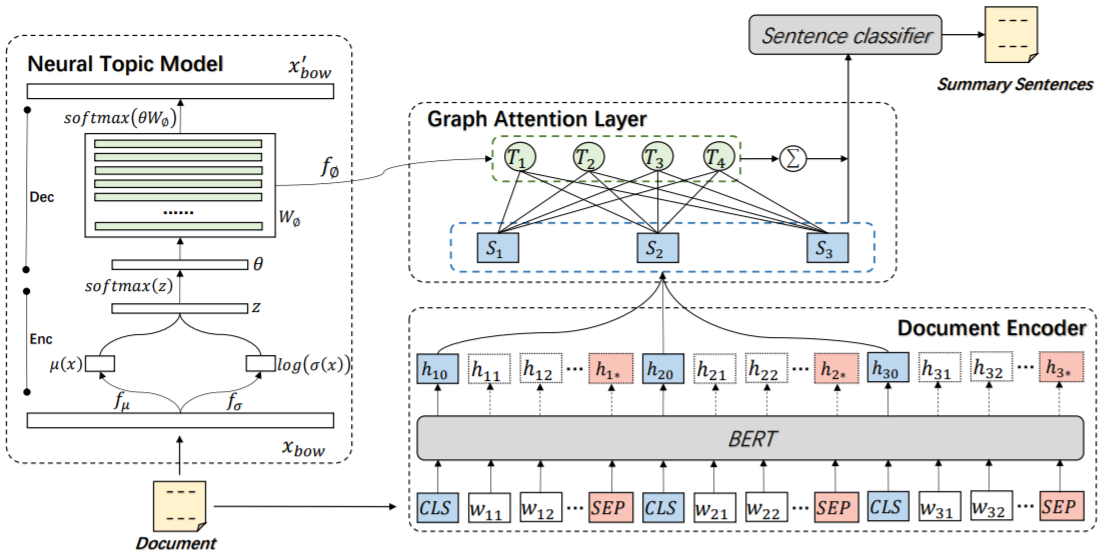
\includegraphics[width=.75\textwidth]{pics/Topic-GraphSum.PNG}
	\caption{Overview of Topic-GraphSum}
	\label{fig:topic_grpah_sum}
\end{figure}

如Fig.\ref{fig:topic_grpah_sum}所示,Topic-GraphSum模型主要分为三个部分,NTM(Neural Topic Model)用于从文档中抽取话题,Document Encoder用于生成每个句子的一个表征,再用前两部生成的topics和句子构造一个Heterogeneous Graph,使用GAT对该异构图进行学习,再将每个句子的表征输入到Sentecnce Classifer中,输出每个句子是否在Summarization中。

\subsection{Editing Graphs to Satisfy Diversity Requirements}
\begin{center}
	\begin{tabular}{rp{6cm}lp{10cm}}%{rl}
		% after \\: \hline or \cline{col1-col2} \cline{col3-col4} ...
		%论文地址:& \href{https://arxiv.org/abs/2010.06253}{https://arxiv.org/abs/2010.06253} \\
		%源码地址:& \href{https://github.com/mocherson/Exp_GNN}{ExpGNN} \\
		关键词:& \textbf{Additional Edges, Graph Editing Problem, Graph Edit Operations, General Factor Problem, Allowable Edit } \\
		写于:& \date{2020-10-20}
	\end{tabular}
\end{center}
论文大意:图中每个结点,其邻居数量处于某个区间内,通过边的增加/删除来将一个图转化为另一个图。

\subsection{On the exact computation of the graph edit distance}
\begin{center}
	\begin{tabular}{rp{6cm}lp{10cm}}%{rl}
		% after \\: \hline or \cline{col1-col2} \cline{col3-col4} ...
		%论文地址:& \href{https://arxiv.org/abs/2010.06253}{https://arxiv.org/abs/2010.06253} \\
		%源码地址:& \href{https://github.com/mocherson/Exp_GNN}{ExpGNN} \\
		关键词:& \textbf{Graph edit distance, Exact algorithms, Integer programming}\\
		写于:& \date{2020-10-20}
	\end{tabular}
\end{center}
论文对几个主流的GED精确/近似算法进行了总结,并在这些算法的基础上进行了一定的改进。但依然是一个精确的GED求解方法。并证明了当图的结点数超过16时,算法将难以运行下去。


\subsection{Retrieval-Augmented Generation for Code Summarization via Hybrid GNN}
\begin{center}
	\begin{tabular}{rp{16cm}lp{20cm}}%{rl}
		
		% after \\: \hline or \cline{col1-col2} \cline{col3-col4} ...
		
		论文地址:& \href{https://openreview.net/pdf?id=zv-typ1gPxA}{https://openreview.net/pdf?id=zv-typ1gPxA} \\
		来源:& ICLR, 2021 \\
		作者:& Shangqing Liu, et al. \\
		%源码:& \href{https://github.com/IBM/EvolveGCN}{EvolveGCN} \\
		
		%  slides:& \href{http://yunshengb.com/wp-content/uploads/2017/03/nips_2018_r2l_workshop_talk.pdf}{{\footnotesize Convolutional Set Matching for Graph Similarity}}\\
		
		关键词:& \textbf{GNN, Code Summarization} \\
		
		写于:& \date{2021-07-19}
		
	\end{tabular}
\end{center}
该论文\cite{liu2021retrieval-augmented}的目标:给定某种语言编写的函数代码,生成这个函数的自然语言描述。自动的代码摘要主要有两张方式:1)Retrieval-based(抽取式);2)Generation-based(生成式)。该论文提出了一种结合这两种方法的增强的抽取式方机制来进行代码总结。
\begin{figure}[h]
	\centering
	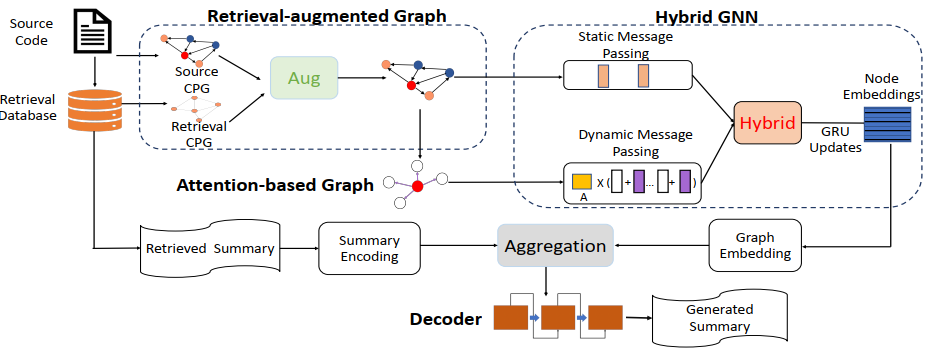
\includegraphics[width=.8\textwidth]{pics/HGNN.png}
	\label{fig:hgnn}
	\caption{Overview of HGNN}
\end{figure}

论文提出的方法是Hybrid GNN(Fig.\ref{fig:hgnn}),首先根据代码的抽象语法树表示成Graph(Fig.\ref{fig:cpg}),再从代码数据集中找到与当前代码最相似的代码(除去当前的函数)及对应的summarization,当前代码的Graph经过最相似的代码的Graph增强后得到static graph,经过注意力机制后生成dynamic graph,在static/dynamic graph上进行message passing,再通过Hybrid massage passing(即将同一个结点在static和dynamic graph中的表征融合后再进行massage passing)。除此之外,还会利用找到的最相似的代码的summarization的表征,将最终得到的结点表征与summarization表征进行拼接后输入基于注意力的LSTM,得到目标代码的表征。

\begin{figure}[h]
	\centering
	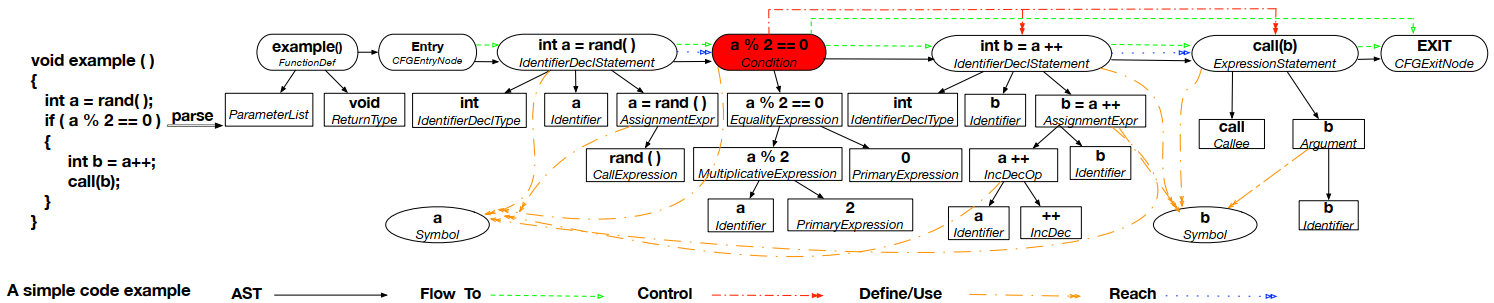
\includegraphics[width=.8\textwidth]{pics/CPG.png}
	\label{fig:cpg}
	\caption{An Example of Code Property Graph(CPG)}
\end{figure}

